% Example LaTeX document for GP111 - note % sign indicates a comment
\documentclass[12pt,a4paper,oneside]{article}
\usepackage{lmodern}
\usepackage[french]{babel}
\usepackage[T1]{fontenc}
\usepackage[utf8]{inputenc}
\usepackage{graphicx}
\usepackage{hyperref}
\usepackage{float}
\usepackage{verbatim}
\usepackage[ruled,vlined]{algorithm2e}
%\usepackage[backend=bibtex,style=verbose-trad2,natbib=true]{biblatex}
\usepackage{natbib}
\graphicspath{{../images/}}
\usepackage{ccaption}
\usepackage{caption}
\usepackage{subcaption}
\usepackage{listings}
\usepackage{color}
\definecolor{name}{rgb}{0.5,0.5,0.5}

% Default margins are too wide all the way around. I reset them here
\setlength{\topmargin}{-.5in}
\setlength{\textheight}{9in}
\setlength{\oddsidemargin}{.125in}
\setlength{\textwidth}{6.25in}

\hypersetup{
    unicode=false,          % non-Latin characters in Acrobat’s bookmarks
    pdftoolbar=true,        % show Acrobat’s toolbar?
    pdfmenubar=true,        % show Acrobat’s menu?
    pdffitwindow=false,     % window fit to page when opened
    pdfnewwindow=true,      % links in new window
    colorlinks=true,       % false: boxed links; true: colored links
    linkcolor=black,          % color of internal links (change box color with linkbordercolor)
    citecolor=green,        % color of links to bibliography
    filecolor=magenta,      % color of file links
    urlcolor=cyan,          % color of external links
    linktoc=page
}

\definecolor{javared}{rgb}{0.6,0,0} % for strings
\definecolor{javagreen}{rgb}{0.25,0.5,0.35} % comments
\definecolor{javapurple}{rgb}{0.5,0,0.35} % keywords
\definecolor{javadocblue}{rgb}{0.25,0.35,0.75} % javadoc
\definecolor{mygray}{rgb}{0.5,0.5,0.5}

\lstset{language=Java,
basicstyle=\ttfamily,
keywordstyle=\color{javapurple}\bfseries,
stringstyle=\color{javared},
commentstyle=\color{javagreen},
morecomment=[s][\color{javadocblue}]{/**}{*/},
tabsize=2,
showspaces=false,
showstringspaces=false,
breaklines=true,
captionpos=b,
frame=lrtb,
numbers=left,
numbersep=5pt,
numberstyle=\tiny\color{mygray},
stepnumber=2
}

\makeatletter
\DeclareRobustCommand\ttfamily
        {\not@math@alphabet\ttfamily\mathtt
         \fontfamily\ttdefault\selectfont\hyphenchar\font=-1\relax}
\makeatother
\DeclareTextFontCommand{\mytexttt}{\ttfamily\hyphenchar\font=45\relax}

\begin{document}

\begin{titlepage}
\begin{flushright}
           
\includegraphics[scale=0.30]{../images/univorleans.png}\\ 
                      Département Informatique
\end{flushright}
\vspace{20mm}
\begin{center}
\textbf{\huge{Documentation Technique}}\\
\vspace{20mm}
\begin{large}
	\textit{Zo RABARIJAONA}\\
	\textit{Jérémy MOROSI}\\
	\textit{Willy FRANÇOIS}\\
	\textit{Raya DJADLI}
\end{large}

\end{center}
\begin{figure}[b!]
\begin{flushright}
~~\\ ~~\\ ~~\\ ~~\\ ~~\\ ~~\\ ~~\\
\large{Année : 2013-2014}
\end{flushright}
\end{figure}
\end{titlepage}

\newpage

\tableofcontents

\newpage

\section{Analyse}


\subsection{Des applications difficilement modifiables}

Castle Defense, librarie, code natif, attaque héxa, rétro engeneering...


\subsection{L'Application Checkers}

l'application Checkers (principe), décompilation, un bytecode obscure
dex2jar, jd-gui, correction des erreurs, éclaircissement du code, une archi mvc.
Fonctionnement de l'appli en interne
\subsubsection{Principe}
\begin{figure}[hp]
	      \begin{center}
		\fbox{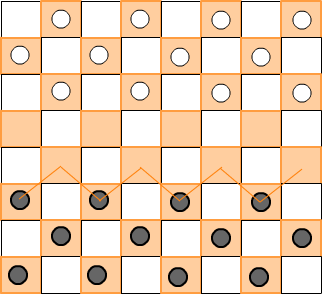
\includegraphics[scale=0.5]{principe}}
	      \end{center}
	\legend{Principe}
\end{figure}
Le jeu est composé de 8 cases sur 8, c’est-à-dire 4 cases en moins que le jeu de dame classique.  Se joue en deux modes : utilisateur contre ordinateur ou utilisateur contre utilisateur.\\
Un joueur peut choisir une couleur (des pions/dames noires ou des pions/dames blanche).  Le jeu est initialement constitué de 3 lignes de 4 pions espacés d’une case. Chaque pion/dame peut se déplacer en diagonale. 
Un pion se transforme en une dame (K) lorsqu’il arrive à la dernière ligne du camp de l’adversaire. Une dame ou un pion peut faire une prise en faisant un déplacement en diagonal. Mais une dame possède l’avantage de traverser plusieurs lignes vide.\\
Un joueur est désigné gagnant si l’adversaire ne possède plus de dames ou de pions.

\subsubsection{Décompilation et analyse du code}

Afin de pouvoir analyser le code de l'application plus aisément, nous avons dû trouver un moyen de décompiler l'application vers du code java.
Pour ce faire, nous avons utilisé \textit{dex2jar} \cite{dex2jar},
une api permettant de décompiler un fichier apk en un fichier jar contenant des fichiers class.
Ensuite, nous avons dû utiliser \textit{jd-gui} \cite{jdgui} sur ce fichier jar pour en afficher le code source.
L'application permet d'exporter les sources ainsi décompilées.

Une fois le code java de l'application en notre possession, nous avons pu commencer à l'analyser.
Nous avons vite remarqué que le code avait été obscurcit avant d'être compilé par le développeur de l'application.
Cela signifie que toutes variables et fonctions avaient un nom sans aucun sens, ce qui gêna la compréhension du code.
Nous avons aussi remarqué que la décompilation c'était mal passée à cause de return et de break à des endroits incongrus.
Nous avons donc commencé par supprimer ces erreurs afin de pouvoir avoir un code "compilable" sous Eclipse.
Ceci nous a offert un accès à l'outil de refactorisation de code pour renommer les variables après avoir compris à quoi elles pouvaient servir.

Malgré cela, à cause du problème de décompilation, certaines méthodes n'avaient aucun sens.
Nous avons donc décidé de relire le code smali des méthodes correspondantes afin de le traduire manuellement en java et ainsi avoir le code original exact.

\subsubsection{Architecture}
Dans un point de vue général, le développeur du jeu Checkers a adopté une architecture MVC. Ce qui nous a beaucoup aidé à determiner les différentes 
classes. 
\begin{figure}[hp]
	      \begin{center}
		\fbox{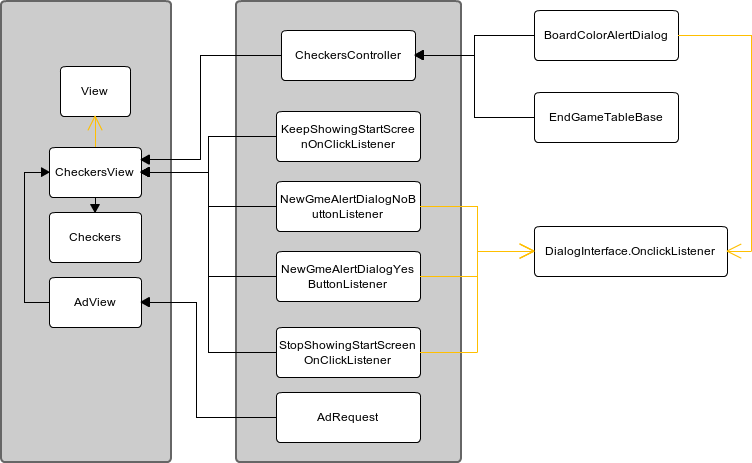
\includegraphics[scale=0.6]{archi}}
	      \end{center}
	\legend{architecture}
\end{figure}
La classe Checkers est la classe principale de l’application.
La classe CherckersView (b.smali) hérite de la classe android.view.View qui gére les vues de l’application. La classe AdView gère la vue pour la publicité.
CheckersController (a.smali) est le controleur principal de l’application. Les classes KeepShowingStartScreenOnclickListener (e.smali), NewGameAlertDialogNoButtonListener (d.smali), NewGameAlertDialogYesButtonListener (c.smali) et StopShowingStartScreenOnclickListener (f.smali) implémente l'interface DialogInterface.OnclickListener sont les classes qui gère les clics.
AdRequest est la classe qui est responsable du chargement de la publicité.


\section{Modifications apportées à l'Application}


\subsection{Suppression de la publicité}
Nous avons remarqué que l'application possède une seule point d'entrée pour afficher la publicité.
L'application charge la vue pour la publicité dans la méthode onCreat().
\begin{figure}[hp]
	      \begin{center}
		\fbox{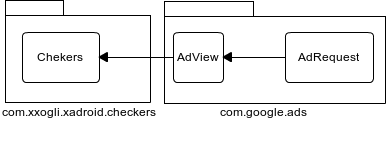
\includegraphics[scale=0.7]{pub}}
	      \end{center}
	\legend{Affichage de la publicité}
\end{figure}

\begin{table}[here]
    \begin{center}
	\begin{tabular}{|l|}
	\hline
	const/16 v1, 0x50 \\[0.2cm]
	
	invoke-virtual {v0, v1}, Lcom/google/ads/AdView;->setGravity(I)V \\[0.2cm]

	new-instance v1, Lcom/google/ads/AdRequest; \\[0.2cm]

	invoke-direct/range {v1 .. v1}, Lcom/google/ads/AdRequest;-><init>()V \\[0.2cm]

	invoke-virtual {v0, v1}, Lcom/google/ads/AdView;->loadAd(Lcom/google/ads/AdRequest;)V \\
	\hline
	\end{tabular}
    \end{center}
    \caption{\label{}code smali pour la publicité}
\end{table} 
La variable v1 contient l'instance de la classe \textit{com.google.ads.AdRequest} qui est le point d'entrée de la publicité dans l'application.
La variable v0 est la vue \textit{com.google.ads.AdView} associée à la publicité. Le chargement de la publicité ce fait par la méthode \textit{loadAd(AdRequest adrequest)}.


\subsection{Ajout d'un bouton Exit}

Beaucoup d'applications n'ayant pas de bouton "Quitter" explicite et ne proposant parfois même pas de quitter (sans faire le bouton Home),
nous avons voulu en ajouter un dans le menu de l'application.

Pour cela, il a fallu modifier les méthodes onCreateOptionsMenu et onOptionsItemSelected de la classe \textit{Checkers}
afin de pouvoir ajouter le bouton et son action.

\begin{figure}[!h]
\begin{verbatim}
    const/4 v9, 0x7
...
    const-string v0, "Undo"
    invoke-interface {p1, v5, v4, v4, v0},
        Landroid/view/Menu;->add(IIILjava/lang/CharSequence;)
        Landroid/view/MenuItem;
    const-string v0, "Exit"
    invoke-interface {p1, v5, v9, v6, v0},
        Landroid/view/Menu;->add(IIILjava/lang/CharSequence;)
        Landroid/view/MenuItem;
    const-string v0, "Switch Side"
\end{verbatim}
    \caption{Ajout du bouton dans onCreateOptionsMenu}
\end{figure}

Lors de l'appui sur le bouton, un appel à la méthode finish() est exécuté.
Ainsi, les méthodes onPause (sauvegardant les données) et onStop (exécutant un System.exit()) sont appelées.

\begin{figure}[!h]
\begin{verbatim}
    const/16 v5, 0x7
...
    :cond_2
    if-ne v1, v3, :cond_42 # On va au test pour le bouton Exit
...
    :cond_42
    if-ne v1, v5, :cond_3 # On retourne au test suivant
    invoke-super {p0}, Landroid/app/Activity;->finish()V
    goto :goto_0
    :cond_3
\end{verbatim}
    \caption{Action du bouton dans onOptionsItemSelected}
\end{figure}


\subsection{Commencer avec des Dames}



\subsection{Choisir le placement des pions}

Après avoir modifié le placement des pions de manière statique dans le code, nous avons voulu aller plus loin en donnant la possibilité au joueur de choisir ce placement. Nous savions déjà quel endroit du code il fallait modifier pour changer les pions à la création d'une nouvelle partie, il fallait juste réussir à modifier la boîte de dialogue qui demande confirmation au joueur lorsque l'on choisit `New Game' dans le menu. Nous voulions que cette boîte de dialogue contienne deux champs de saisie supplémentaires (un pour les pions blancs et un pour les noirs) dans lesquels l'utilisateur puisse saisir une suite de douze `0' et/ou `1', et qu'en cliquant sur `Yes' pour lancer la nouvelle partie, le plateau soit initialisé avec des pions normaux là où les champs contiennent des `0', et des dames là où ils contiennent des `1'.\\

Pour ce faire, l'idée était de faire un vrai projet Android pour pouvoir créer et tester facilement une boîte de dialogue, puis d'exporter le projet en \mytexttt{.apk}, décompiler cet \mytexttt{.apk}, récupérer le code de la boîte de dialogue dans le fichier \mytexttt{.smali} correspondant, et le mettre à la place du code de la vraie boîte de dialogue du jeu.

Nous avons donc fait un projet Android contenant les classes \mytexttt{b} (listing \ref{lstPlacementB}) et \mytexttt{a} (listing \ref{lstPlacementA}), ainsi qu'une classe \mytexttt{MainActivity} présente uniquement pour pouvoir lancer l'application et tester la boîte de dialogue. La classe \mytexttt{b} correspond à la classe \mytexttt{CheckersView} qui est la vue du jeu, et la classe \mytexttt{a} correspond à la classe \mytexttt{CheckersController} qui est le contrôleur. \`{A} noter que certaines lignes de la classe \mytexttt{b} ont été retirées (comme l'affectation du layout pour les éléments de la boîte de dialogue ou le constructeur) afin de la simplifier.\\

On peut remarquer plusieurs choses. Tout d'abord, nous avons gardé les noms des packages, classes, variables ainsi que les signatures des fonctions tels qu'ils apparaissent dans les fichiers \mytexttt{.smali} du jeu pour pouvoir injecter notre code sans trop de problèmes. Par contre, pour les fonctions et variables supplémentaires qui ne sont utilisées que par notre code, nous avons mis des vrais noms puisque ça ne pose pas de problème.

Ensuite, la méthode \mytexttt{a} de la classe \mytexttt{b} ne fait que retourner \mytexttt{false}. Cette méthode est uniquement présente pour pouvoir compiler le code puisque l'on doit y faire appelle quand l'utilisateur confirme la nouvelle partie. Quant à la méthode \mytexttt{a} de la classe \mytexttt{a} qui doit initialiser le plateau, elle ne contient que le code à compiler et à injecter dans la méthode originale.\\

Pour entrer plus en détail dans le code, et plus précisément la classe \texttt{b}, on a les quatres variables \mytexttt{newGame(White|Black)(Pieces|Kings)Placement} (ligne 9) qui contiennent les positions des pions normaux et des dames pour les deux joueurs. On peut voir que, par défaut, la variable \mytexttt{newGameWhitePiecesPlacement} contient un entier avec les douzes premiers bits à `1', et que la variable \mytexttt{newGameBlackKingsPlacement} contient un entier avec les douzes derniers bits `1'.

Le jeu utilise des entiers pour représenter le plateau. Les douzes premiers bits correspondent aux trois premières rangées, les douzes derniers aux trois dernières, le premier bit est la case tout en haut à gauche, et le dernier est la case tout en bas à droite. C'est pour ça que l'on fait des opérations étranges (ligne 50 et lignes 64 à 69) sur la saisie de l'utilisateur.

Pour ce qui est de la classe \texttt{a}, on assigne simplement les valeurs de nos variables aux vraies positions des pions avant l'initialisation du plateau (lignes 14 à 17).\\

Une fois notre \texttt{.apk} généré et le code de notre application Android décompilé, on peut très simplement injecter notre code dans les \texttt{.smali} du jeu.\\

\begin{lstlisting}[caption=b.java (CheckersView.java), label=lstPlacementB]
package com.xxogli.xadroid.checkers;

// CheckersView
public class b extends View {

	private Context a;
	private a p;		// CheckersController
	
	public int newGameWhitePiecesPlacement = 4095;
	public int newGameWhiteKingsPlacement = 0;
	public int newGameBlackPiecesPlacement = 0;
	public int newGameBlackKingsPlacement = -1048576;

	private TextView textView(String s) {
		TextView tv = new TextView(a);
		tv.setText(s);
		return tv;
	}
	
	private EditText editText(String s) {
		EditText et = new EditText(a);
		et.setText(s);
		return et;
	}
	
	private TableRow tableRow(String s, EditText et) {
		TableRow tr = new TableRow(a);
		tr.addView(textView(s));
		tr.addView(et);
		return tr;
	}
	
	private TableLayout tableLayout(TableRow ...rows) {
		TableLayout tl = new TableLayout(a);
		for(TableRow tr : rows) {
			tl.addView(tr);
		}
		return tl;
	}
	
	private LinearLayout linearLayout(View ...views) {
		LinearLayout ll = new LinearLayout(a);
		for(View v : views) {
			ll.addView(v);
		}
		return ll;
	}

	private int value(EditText et) {
		return Integer.parseInt(new StringBuilder(et.getText().toString()).reverse().toString(), 2);
	}
	
	// newGameDialog
	public void f() {
		AlertDialog.Builder b = new AlertDialog.Builder(a);
		final EditText et1 = editText("000000000000");
		final EditText et2 = editText("000000000000");
		b.setView(tableLayout(
			tableRow("White:", et1), tableRow("Black:", et2)
		)).setMessage("Start a new game?")
		.setCancelable(false)
		.setPositiveButton("Yes", new OnClickListener() {
			public void onClick(DialogInterface dialog, int which) {
				int i = value(et1);
				newGameWhitePiecesPlacement = ~i & 0xFFF;
				newGameWhiteKingsPlacement = i & 0xFFF;
				i = value(et2) << 20;
				newGameBlackPiecesPlacement = ~i & 0xFFF00000;
				newGameBlackKingsPlacement = i & 0xFFF00000;
				a(false, -1, 0, 0, 0);
				postInvalidate();
			}
		})
		.setNegativeButton("No", new OnClickListener() {
			public void onClick(DialogInterface dialog, int which) {
			}
		}).show();
	}
	
	// gameStatus
	private final boolean a(boolean b, int m, int v, int d, int n) {
		return false;
	}

}
\end{lstlisting}

\begin{lstlisting}[caption=a.java (CheckersController.java), label=lstPlacementA]
package com.xxogli.xadroid.checkers;

// CheckersController
public class a {

	private b j;		// CheckersView
	private int d;	// lastWhitePiecesPlacement
	private int e;	// lastWhiteKingsPlacement
	private int f;	// lastBlackPiecesPlacement
	private int g;	// lastBlackKingsPlacement

	// initPlateau
	public final void a() {
		this.d = j.newGameWhitePiecesPlacement;
		this.e = j.newGameWhiteKingsPlacement;
		this.f = j.newGameBlackPiecesPlacement;
		this.g = j.newGameBlackKingsPlacement;
	}

}
\end{lstlisting}

\subsection{Échanger pions et dames à changement de joueur}

Dans cette section, nous avons ajouté une option qui nous permet d'avoir le choix d'échanger 
des jetons noirs et blancs en pions ou dames.


\begin{figure}[hp]
	      \begin{center}
			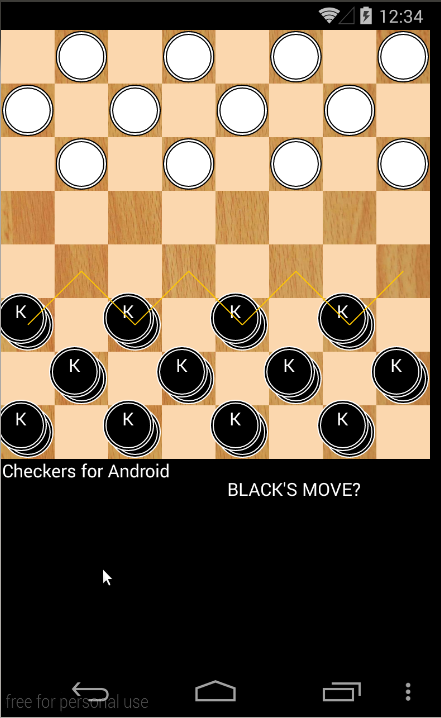
\includegraphics[width=0.4\textwidth]{state0}
	      \end{center}
	\caption{Avant modification}
\end{figure}
Pour celà nous avons d'abord ajouté une option "Switcher les Dames" dans le menu "Options". 
\begin{figure}[h!]
	      \begin{center}
			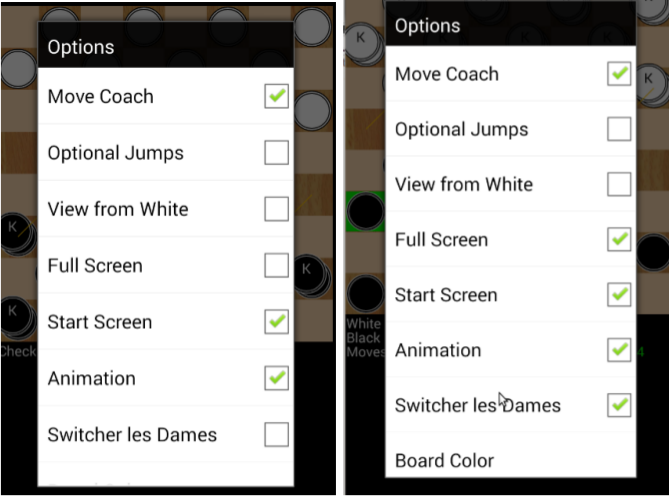
\includegraphics[width=0.8\textwidth]{menu}
		  \end{center}
	\caption{ajout d'une option dans le menu}
\end{figure}
On a effectué cet ajout dans \textit{Chechers.smali} comme on peut le voir sur la Figure 9.\newpage

\begin{figure}[h!]
\begin{verbatim}
    const/4 v1, 0x6
    const/4 v2, 0x6
    const-string v3, "Switcher les Dames"
    invoke-interface {v0, v4, v1, v2, v3}, Landroid/view/SubMenu;->
        add(IIILjava/lang/CharSequence;)Landroid/view/MenuItem;
    move-result-object v1
    invoke-interface {v1, v4}, Landroid/view/MenuItem;->
        setCheckable(Z)Landroid/view/MenuItem;
    move-result-object v1
    iget-object v2, p0, Lcom/xxogli/xadroid/checkers/Checkers;->
        a:Lcom/xxogli/xadroid/checkers/b;
    invoke-virtual {v2, v5}, Lcom/xxogli/xadroid/checkers/b;->
        permuter(Z)Z
    move-result v2
    invoke-interface {v1, v2}, Landroid/view/MenuItem;->
        setChecked(Z)Landroid/view/MenuItem;
    \end{verbatim}
    \caption{Ajout de l'Option dans onCreateOptionsMenu}
\end{figure}


Après avoir ajouté l'option "Switcher les Dames" dans le menu des Options, nous insérons la méthode permuter() qui prend 
un booléen en paramètre et qui renvoie l'état de la variable \textbf{switchdame} qui est un attribut de la "classe b" de type booléen que nous avons ajouté.


\begin{figure}[!hp]
\begin{verbatim}
.method public final  permuter(Z)Z
.locals 1
    if-eqz p1, :cond_0
    iget-boolean v0, p0, Lcom/xxogli/xadroid/checkers/b;->switchdame:Z
    if-eqz v0, :cond_1
    const/4 v0, 0x0
    :goto_0
    iput-boolean v0, p0, Lcom/xxogli/xadroid/checkers/b;->switchdame:Z
    :cond_0
    iget-boolean v0, p0, Lcom/xxogli/xadroid/checkers/b;->switchdame:Z
    return v0
    :cond_1
    const/4 v0, 0x1
    goto :goto_0
.end method
\end{verbatim}
    \caption{Ajout de l'action dans onCreateOptionsMenu}
\end{figure}

Nous avons ensuite ajouté l'action à exécuter lorsqu'on choisit l'option "Switcher les Dames" dans \textit{onOptionsItemSelected}.

\begin{figure}[!hp]
\begin{verbatim}
    :cond_9
    const/4 v2, 0x6
    if-ne v1, v2, :cond_10
    iget-object v1, p0, Lcom/xxogli/xadroid/checkers/Checkers;->
        a:Lcom/xxogli/xadroid/checkers/b;
    invoke-virtual {v1, v0}, Lcom/xxogli/xadroid/checkers/b;->
         permuter(Z)Z
    move-result v1
    invoke-interface {p1, v1}, Landroid/view/MenuItem;->
        setChecked(Z)Landroid/view/MenuItem;
    goto/16 :goto_0
\end{verbatim}
    \caption{Ajout de l'action dans le onOptionsItemSelected}
\end{figure}

\newpage

Le résultat est affiché comme suit.

\begin{figure}[h!]
	      \begin{center}
			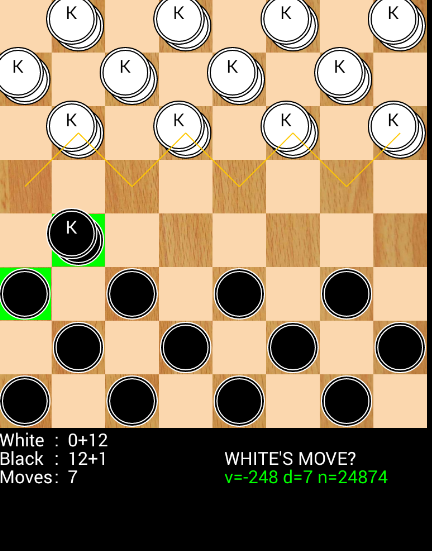
\includegraphics[width=0.4\textwidth]{state1}
	      \end{center}
	\caption{avant modification}
\end{figure}


\paragraph{Remarque:}
Lors de l'execution, nous avons constaté qu'il y avait un soucis avec la permutation.
Ce dernier est dû au au fait que le contrôleur doit prévoir à l'avance le coup qu'il va jouer en fonction
de la position des jetons qu'il a avant d'effectuer le switch.
Ainsi, on se retrouve avec un jeton supplémentaire de l'ancien type.



\appendix

%\bibliography{bibliographie}{}
%\bibliographystyle{plain}
\end{document}
